\vspace{-1mm}
\section{Experimental Evidence} \label{sec:experiments}
\vspace{-1mm}



We primarily study the Transformers-based GPT-2 model with 12 layers and 8 heads per layer. Alternative configurations with fewer heads per layer, or with more layers, also support our findings; we defer them to \S \ref{app:1-head} and \S\ref{app:24-layer}. We initially focus on isotropic cases where $\bSigma = \bI$ and later consider ill-conditioned $\bSigma$ in \S \ref{ssec:ill}. Our training setup is exactly the same as \citet{Garg2022WhatCT}: models are trained with at most $n = 40$ in-context examples for $d = 20$ (with the same learning rate, batch size etc.).  

We claim that Transformers learn high-order optimization methods in-context. We provide evidence that Transformers improve themselves with more layers in \S \ref{ssec:progress}; Transformers share the same rate of convergence as \newton, exponentially faster than that of GD, in \S \ref{ssec:tf_similar_newton}; and they also  perform well on ill-conditioned problems in \S \ref{ssec:ill}. Finally, we contrast  Transformers with LSTMs in \S \ref{ssec:lstm}.


\vspace{-1mm}
\subsection{Transformers improve progressively over layers} \label{ssec:progress}
\vspace{-1mm}

Many known algorithms for linear regression, including GD, OGD, and \newton, are \emph{iterative}:
their performance progressively improves as they perform more iterations, eventually converging to a final solution.
How can a Transformer implement such an iterative algorithm?
\citet{Oswald2022TransformersLI} propose that deeper \emph{layers} of the Transformer may correspond to more iterations;
in particular, they show that there exist Transformer parameters such that each attention layer performs one step of GD.

Following this intuition, we first investigate whether the predictions of a trained Transformer improve as the layer index $\ell$ increases. 
For each layer of hidden states $\bH^{(\ell)}$ (see \cref{def:transformers}), we re-train the \verb|ReadOut| to predict $y_t$ for each $t$; the new predictions are given by $\mathrm{ReadOut}^{(\ell)}\left[\bH^{(\ell)}\right]$. Thus for each input prompt, there are $L$ Transformer predictions parameterized by layer index $\ell$.
All parameters besides the \verb|ReadOut| layer parameters are kept frozen.

As shown in \Cref{subfig:transformers-convergence} (and \cref{subfig:transformers} in the Appendix), as we increase the layer index $\ell$, the prediction performance improves progressively. 
Hence, Transformers progressively improve their predictions over layers $\ell$, similar to how iterative algorithms improve over steps. \new{Such observations are consistent with language tasks where Transformers-based language models also improve their predictions along with layer progressions \citep{geva-etal-2022-transformer,chuang2023dola}.}

\begin{figure*}[t]
    \centering
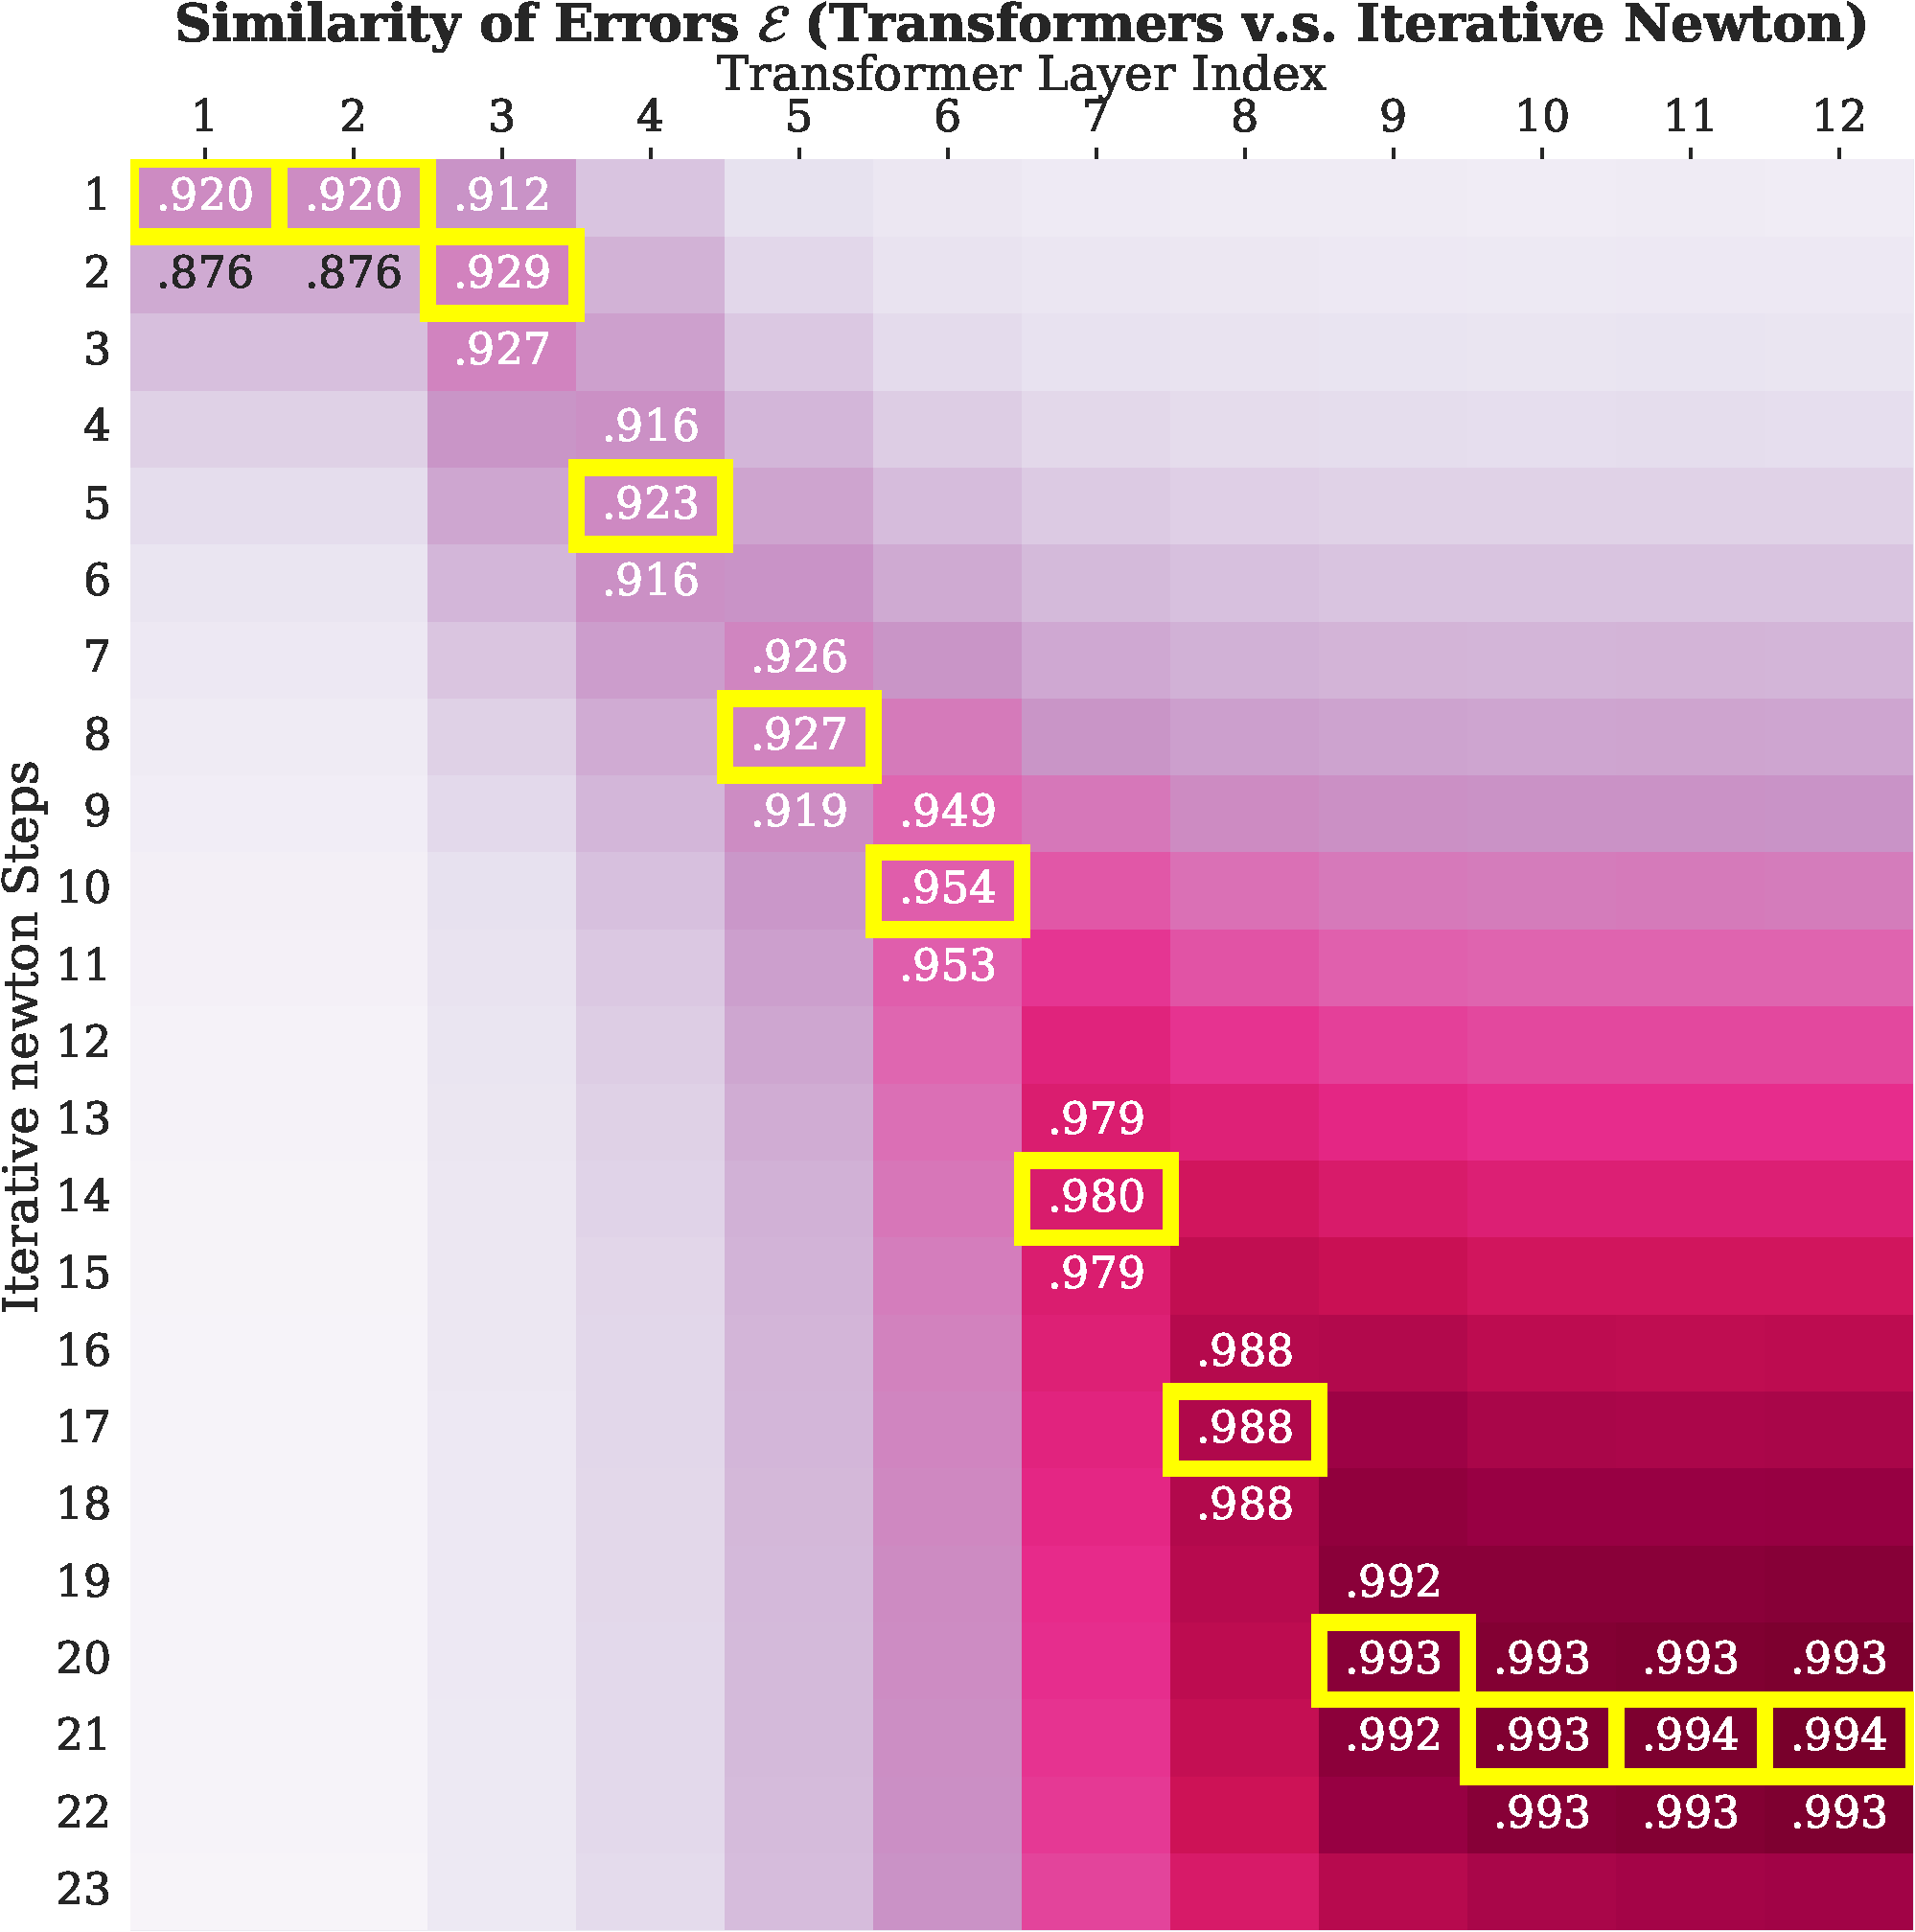
\includegraphics[width=0.49\linewidth]{Figures/heatmaps/resid_sim_heatmap_tf_iterative_newton.pdf}
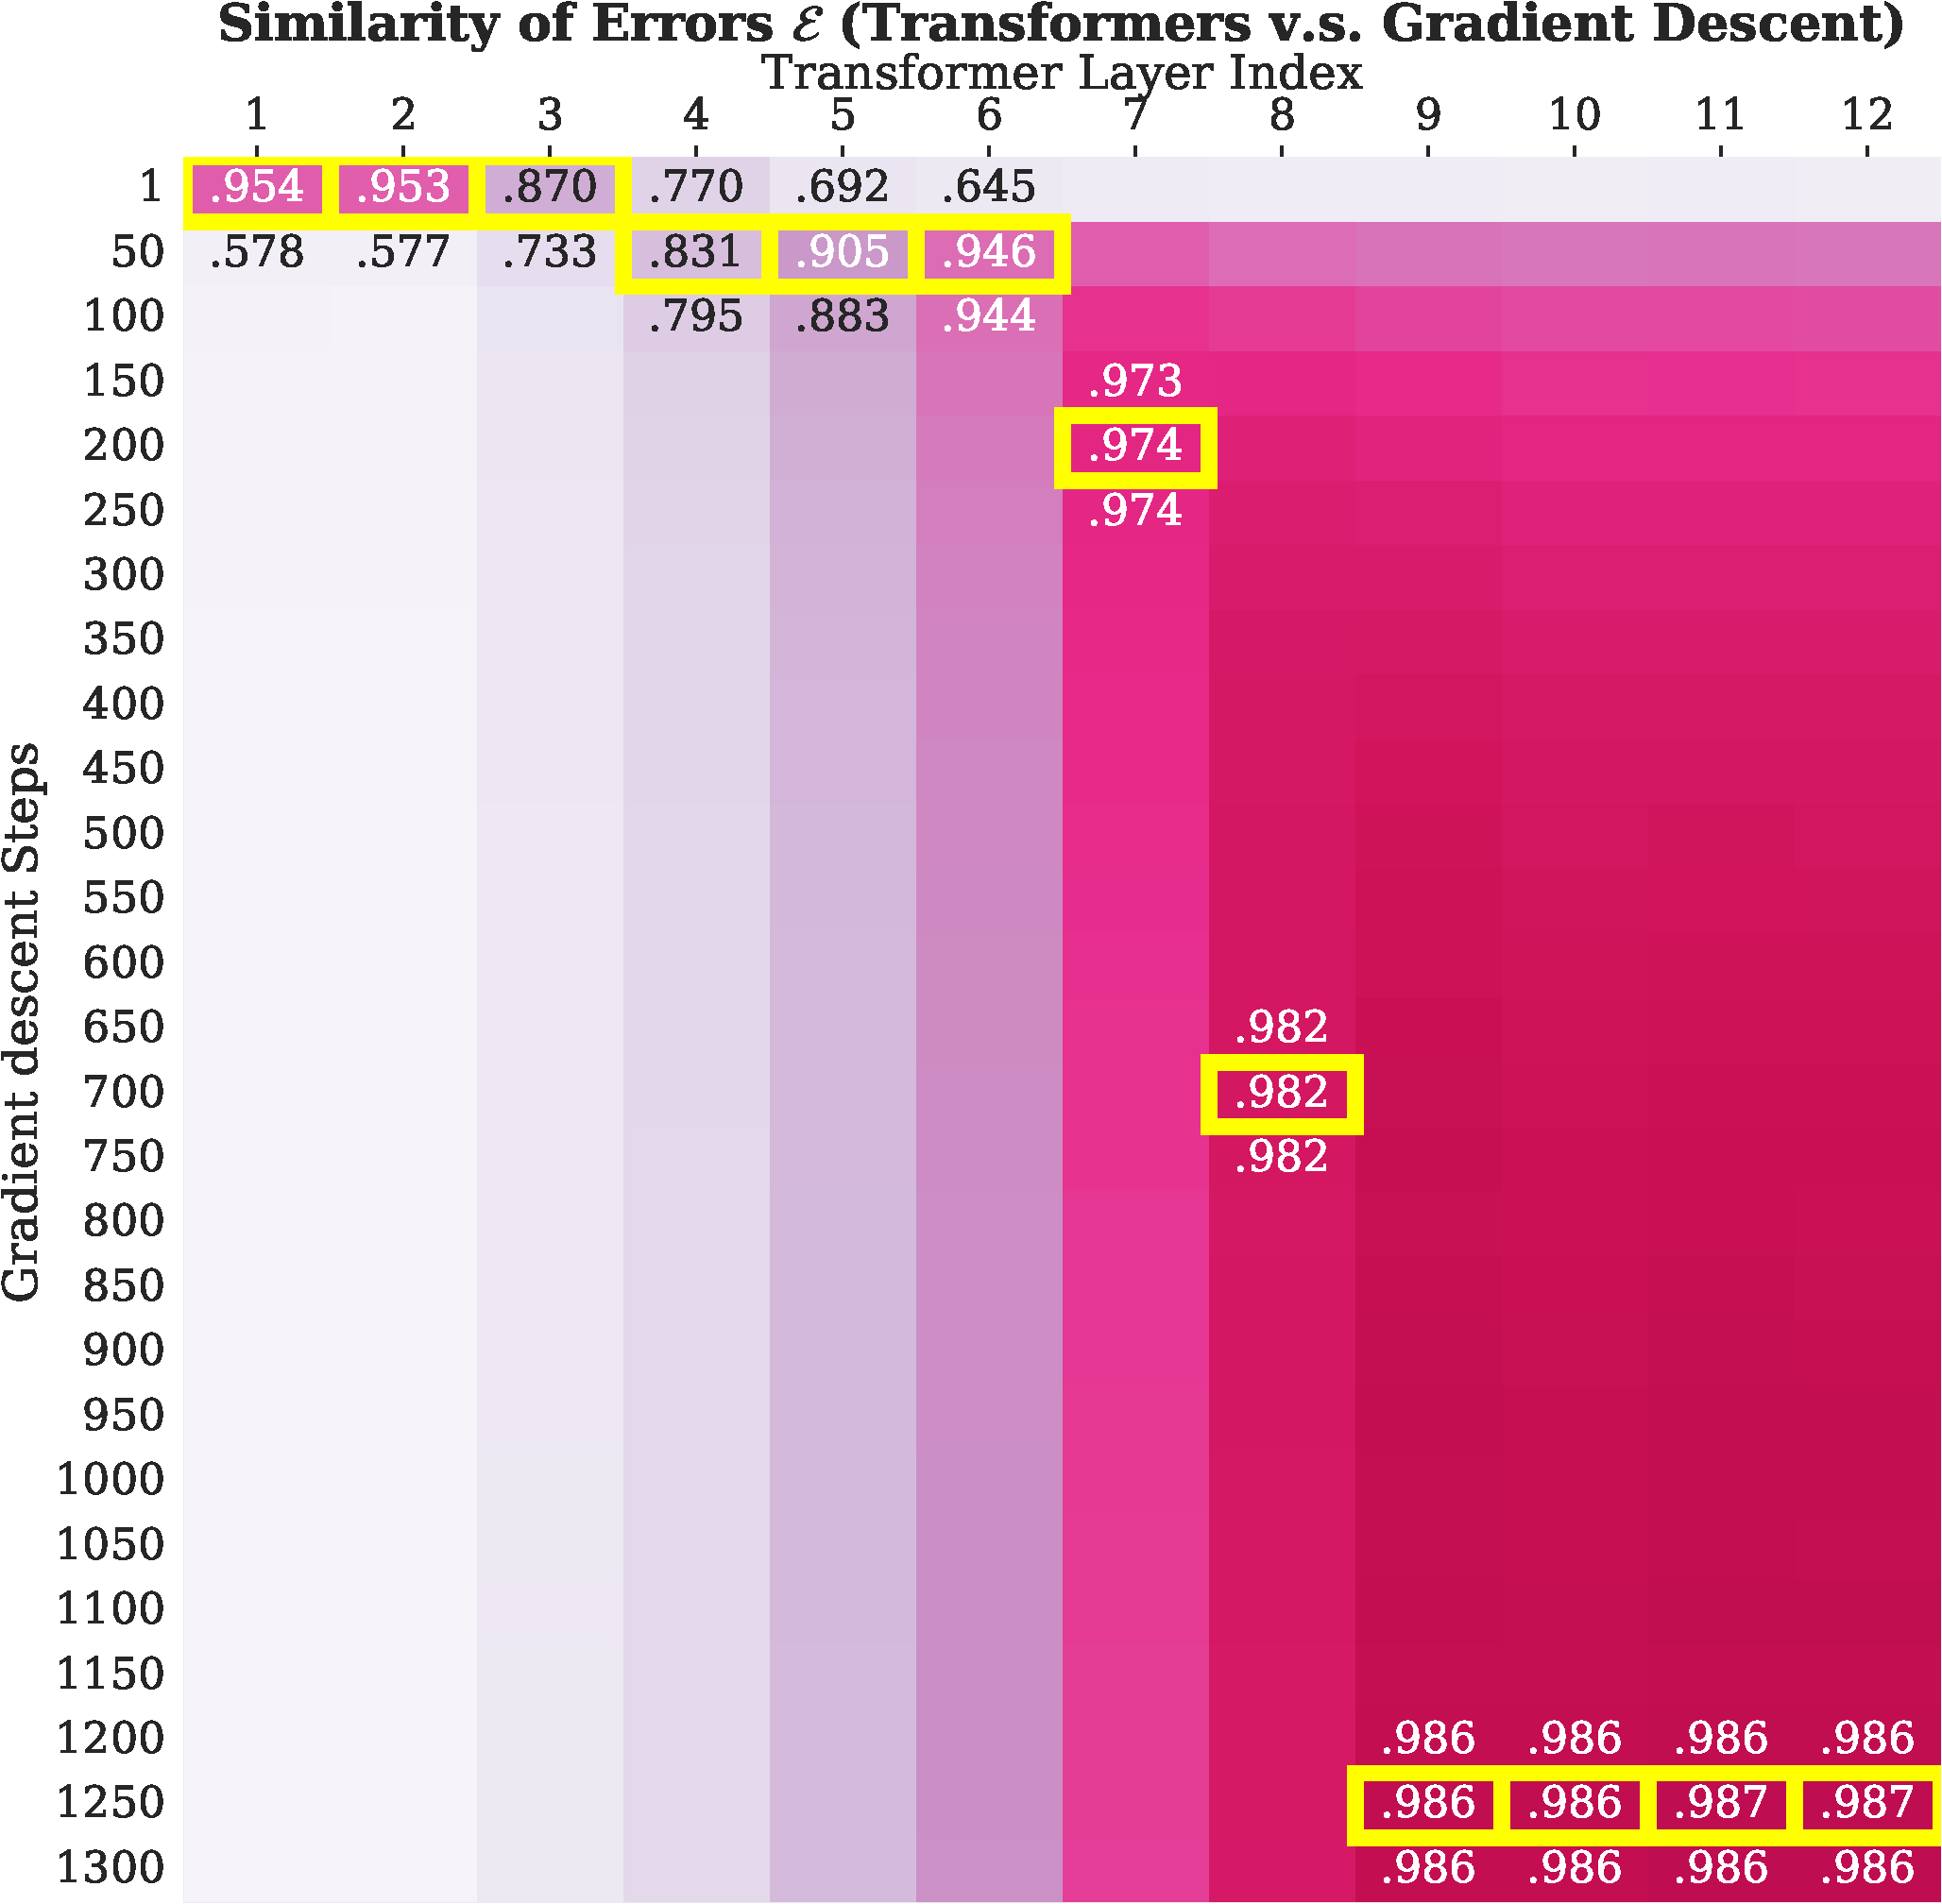
\includegraphics[width=0.49\linewidth]{Figures/heatmaps/resid_sim_heatmap_tf_gradient_descent.pdf}
\caption{\textbf{Heatmaps of Similarity.} The best matching steps are highlighted in yellow. Transformers layers show a linear trend with \newton\ steps but an exponential trend with GD. This suggests Transformers and \newton\ have the same convergence rate that is exponentially faster than GD. See \Cref{fig:gd_heatmap_log_scale} for an additional heatmap where GD's steps are shown in log scale: on that plot there is a linear correspondence between Transformers and GD's steps. This further strengthens the claim that Transformers have an exponentially faster rate of convergence than GD.}
\vspace{-1ex}
\label{fig:heatmap}
\end{figure*}


\vspace{-1mm}
\subsection{Transformers are more similar to second-order methods, such as \newton} \label{ssec:tf_similar_newton}
\vspace{-1mm}

We now test the more specific hypothesis that the iterative updates performed across Transformer layers are similar to the iterative updates for known iterative algorithms. First, \Cref{fig:convergence} shows that the middle layers of Transformers converge at a rate similar to \newton, and faster than GD.
In particular, the Transformer and \newton\ both converge at a superlinear rate, while GD converges at a sublinear rate. 

Next, we analyze whether each layer $\ell$ of the Transformer corresponds to performing $k$ steps of some iterative algorithm, for some $k$ depending on $\ell$.
We focus here on GD\ and \newton's Method; we will discuss online algorithms in \Cref{ssec:lstm}, and additional optimization methods in \Cref{sec:second-order}. We will discuss results on noisy linear regression tasks in \Cref{ssec:noisy}.

For each layer $\ell$ of the Transformer,
we measure the best-matching similarity (see Def.~\ref{def:matching}) with candidate iterative algorithms with the optimal choice of the number of steps $k$.
As shown in \Cref{fig:heatmap}, the Transformer has very high error similarity with \newton's method at all layers.
Moreover, we see a clear \emph{linear} trend between layer 3 and layer 9 of the Transformer, where each layer appears to compute roughly 3 additional iterations of \newton's method.
This trend only stops at the last few layers because both algorithms converge to the OLS solution;
Newton is known to converge to OLS (see \S\ref{ssec:other_methods}), and we verify in \Cref{app:exp_standard} that the last few layers of the Transformer also basically compute OLS (see \Cref{fig:over_examples} in the Appendix). 
We observe the same trends when using similarity of induced weights as our similarity metric (see \Cref{fig:full_heatmap_sim_w} in the Appendix).\Cref{fig:bfgs} in the Appendix shows that there is a similar \textit{linear} trend between Transformer and BFGS, an alternative quasi-Newton method. This is perhaps not surprising, given that BFGS also gets a superlinear convergence rate for linear regression \cite{nocedal1999numerical}.
Thus, we do not claim that Transformers specifically implement \newton, only that they (approximately) implement some second-order method.

In contrast, even though GD\ has a comparable similarity with the Transformers at later layers, their best matching follows an \textit{exponential} trend. As discussed in the \Cref{ssec:other_methods}, for well-conditioned problems where  $\kappa \approx 1$, to achieve $\epsilon$ error, the rate of convergence of GD\ is $\mathcal{O}(\log (1/\epsilon))$ while the rate of convergence of \newton\ is $\mathcal{O}(\log \log (1/\epsilon))$. Therefore the rate of convergence of \newton\ is exponentially faster than GD.  Transformer's \textit{linear} correspondence with \newton\ and its \textit{exponential} correspondence with GD\ provides strong evidence   that the rate of convergence of Transformers is similar to \newton, i.e., $\mathcal O(\log \log (1/\epsilon))$. We also note that it is not possible to significantly improve GD's convergence rate without using second-order methods: \citet{nemirovskii1983problem} showed a $ \Omega\big( \log(1/\epsilon) \big)$  lower bound on the convergence rate of gradient-based methods for smooth and strongly convex problems, and \cite{Arjevani2016OnLower} shows a similar lower bound specifically for quadratic problems. 

In the Appendix, we show that limited-memory BFGS \cite{Liu1989OnTL} and conjugate gradient (see \Cref{fig:conjugate-gradient}), which do not use full-second order information, also converge slower than Transformers. This provides further evidence for the usage of second-order information by Transformers. We also show more evidence by investigating alternative function classes such as linear regression with noises in \Cref{ssec:noisy} and 2-layer neural network with ReLU or Tanh activation function in \Cref{app:non-linear}. 

Overall, we conclude that a Transformer trained to perform in-context linear regression learns to implement an algorithm that is very similar to second-order methods, such as \newton's method, not GD. 
Starting at layer 3, subsequent layers of the Transformer compute more and more iterations of \newton's method.
This algorithm successfully solves the linear regression problem, as it converges to the optimal OLS solution in the final layers.


\begin{figure*}[t]
\centering
    \begin{minipage}[b]{0.32\linewidth}
            \centering
            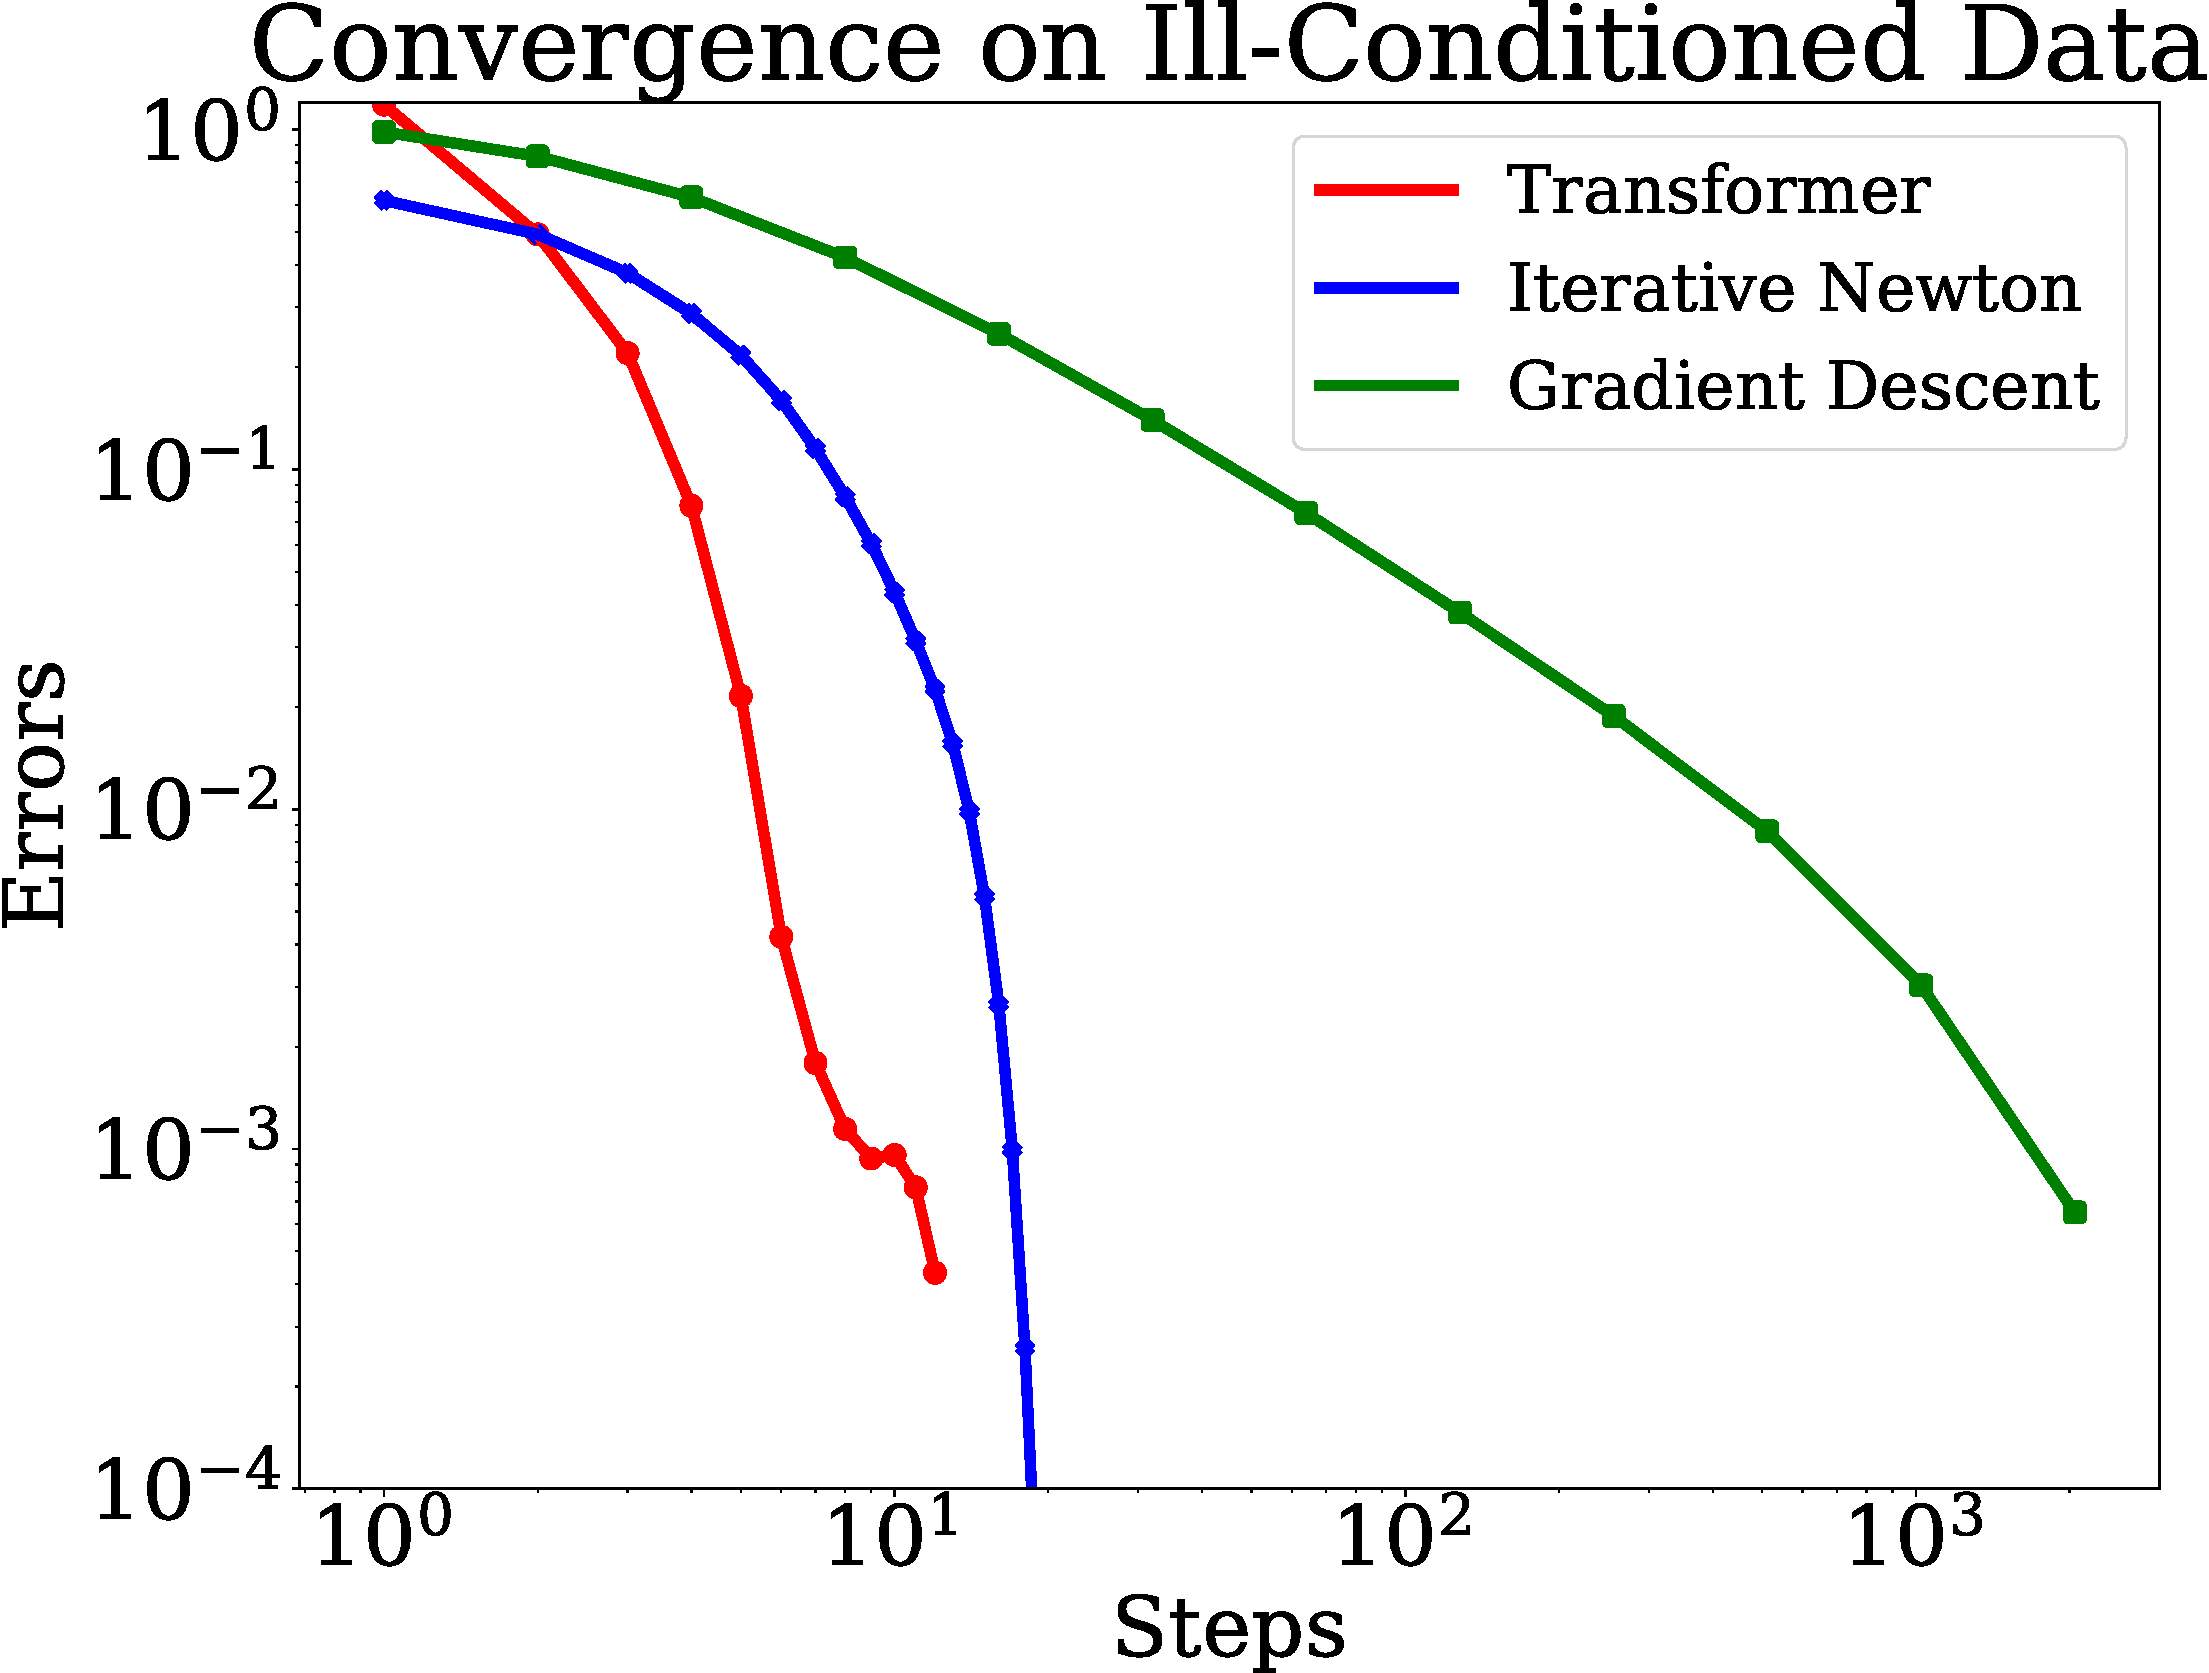
\includegraphics[width=0.95\linewidth]{Figures/convergence/convergence_ill_new2.pdf}
            \vspace{1mm}
            \caption{Transformers performance on ill-conditioned data. Given 40 in-context examples, Transformers and \newton\ converge similarly and they both can converge to the OLS solution quickly whereas GD\ suffers.}
            \label{fig:ill}
    \end{minipage}
    \hfill
    \begin{minipage}[b]{0.65\linewidth}
    \centering
    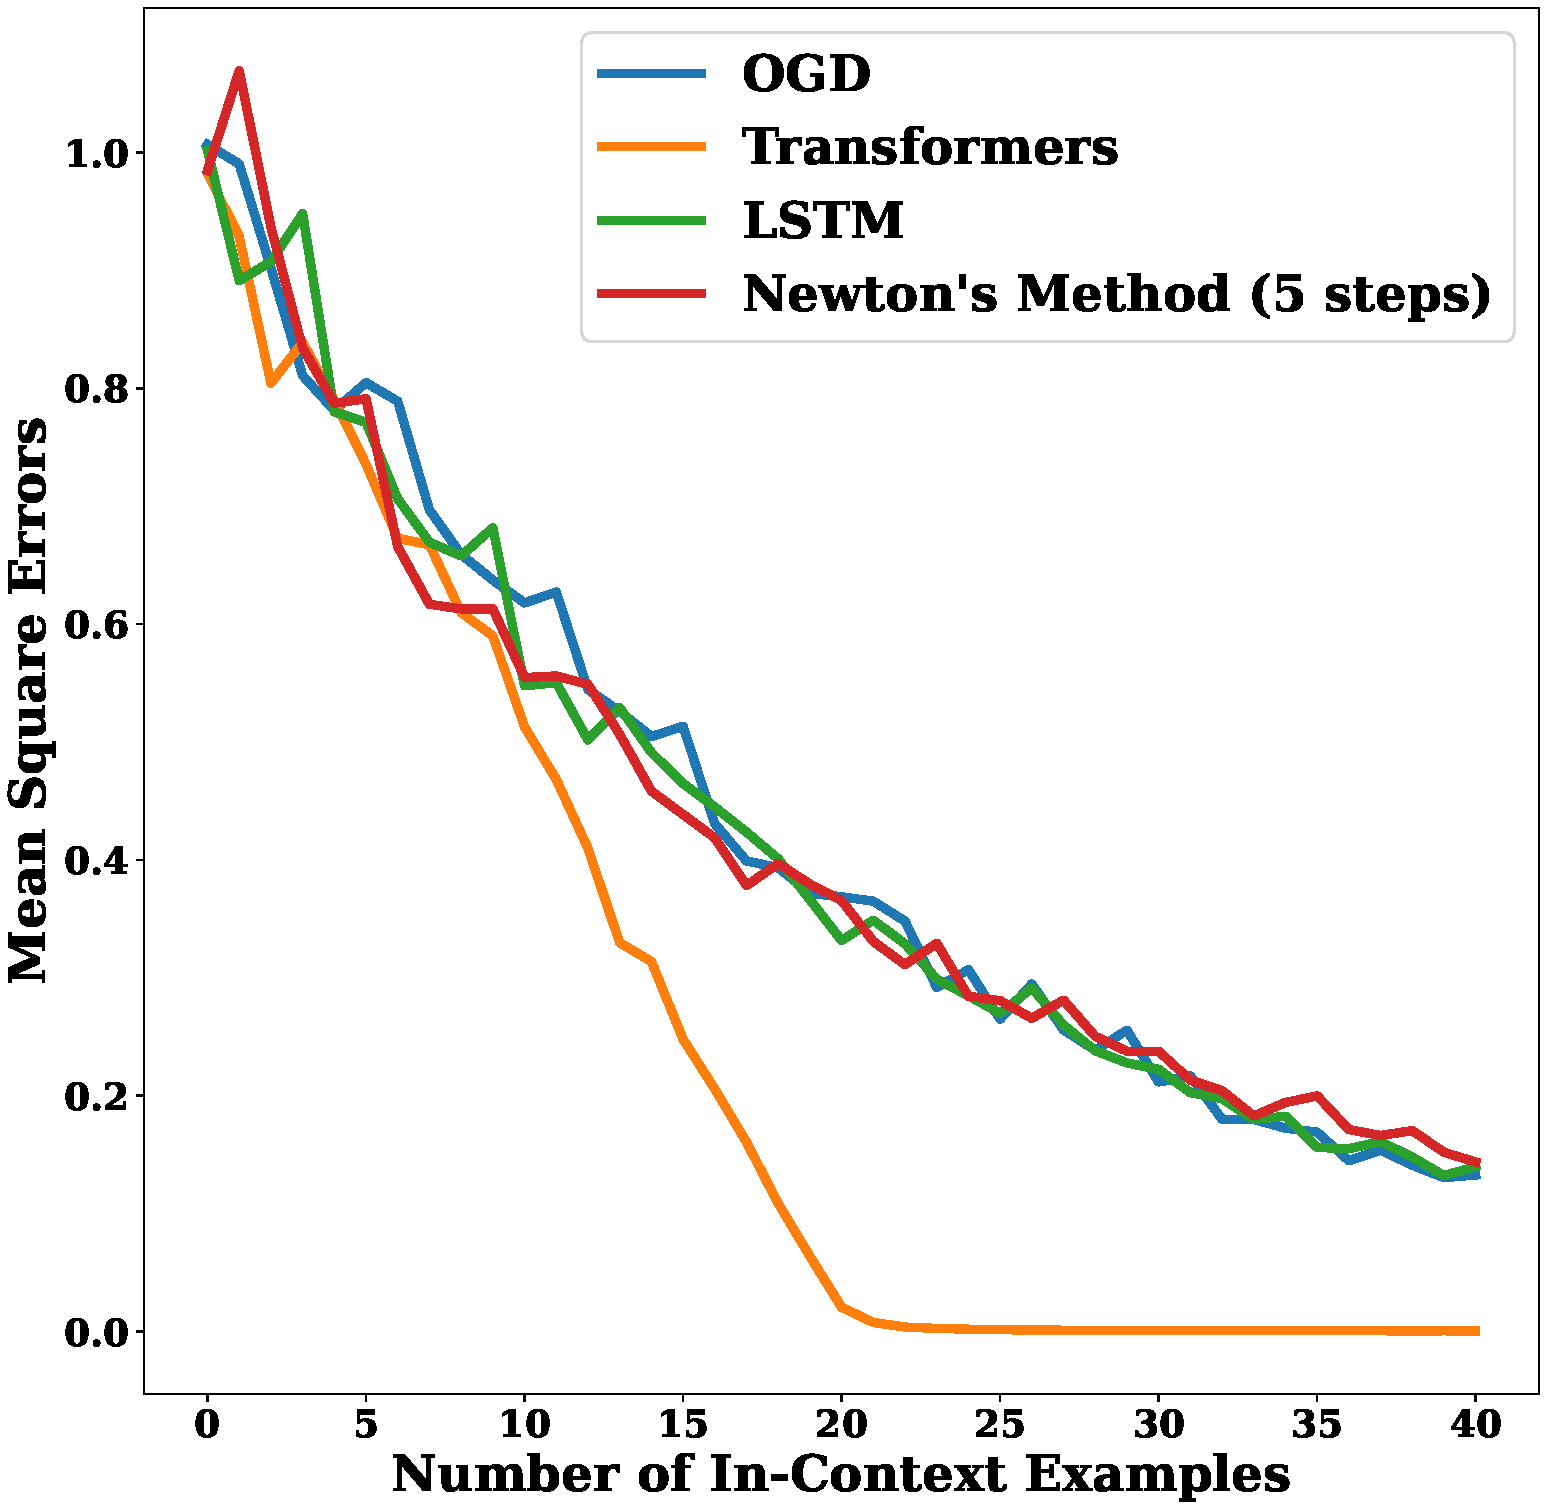
\includegraphics[width=0.42\linewidth]{Figures/lstm_compare.pdf}
    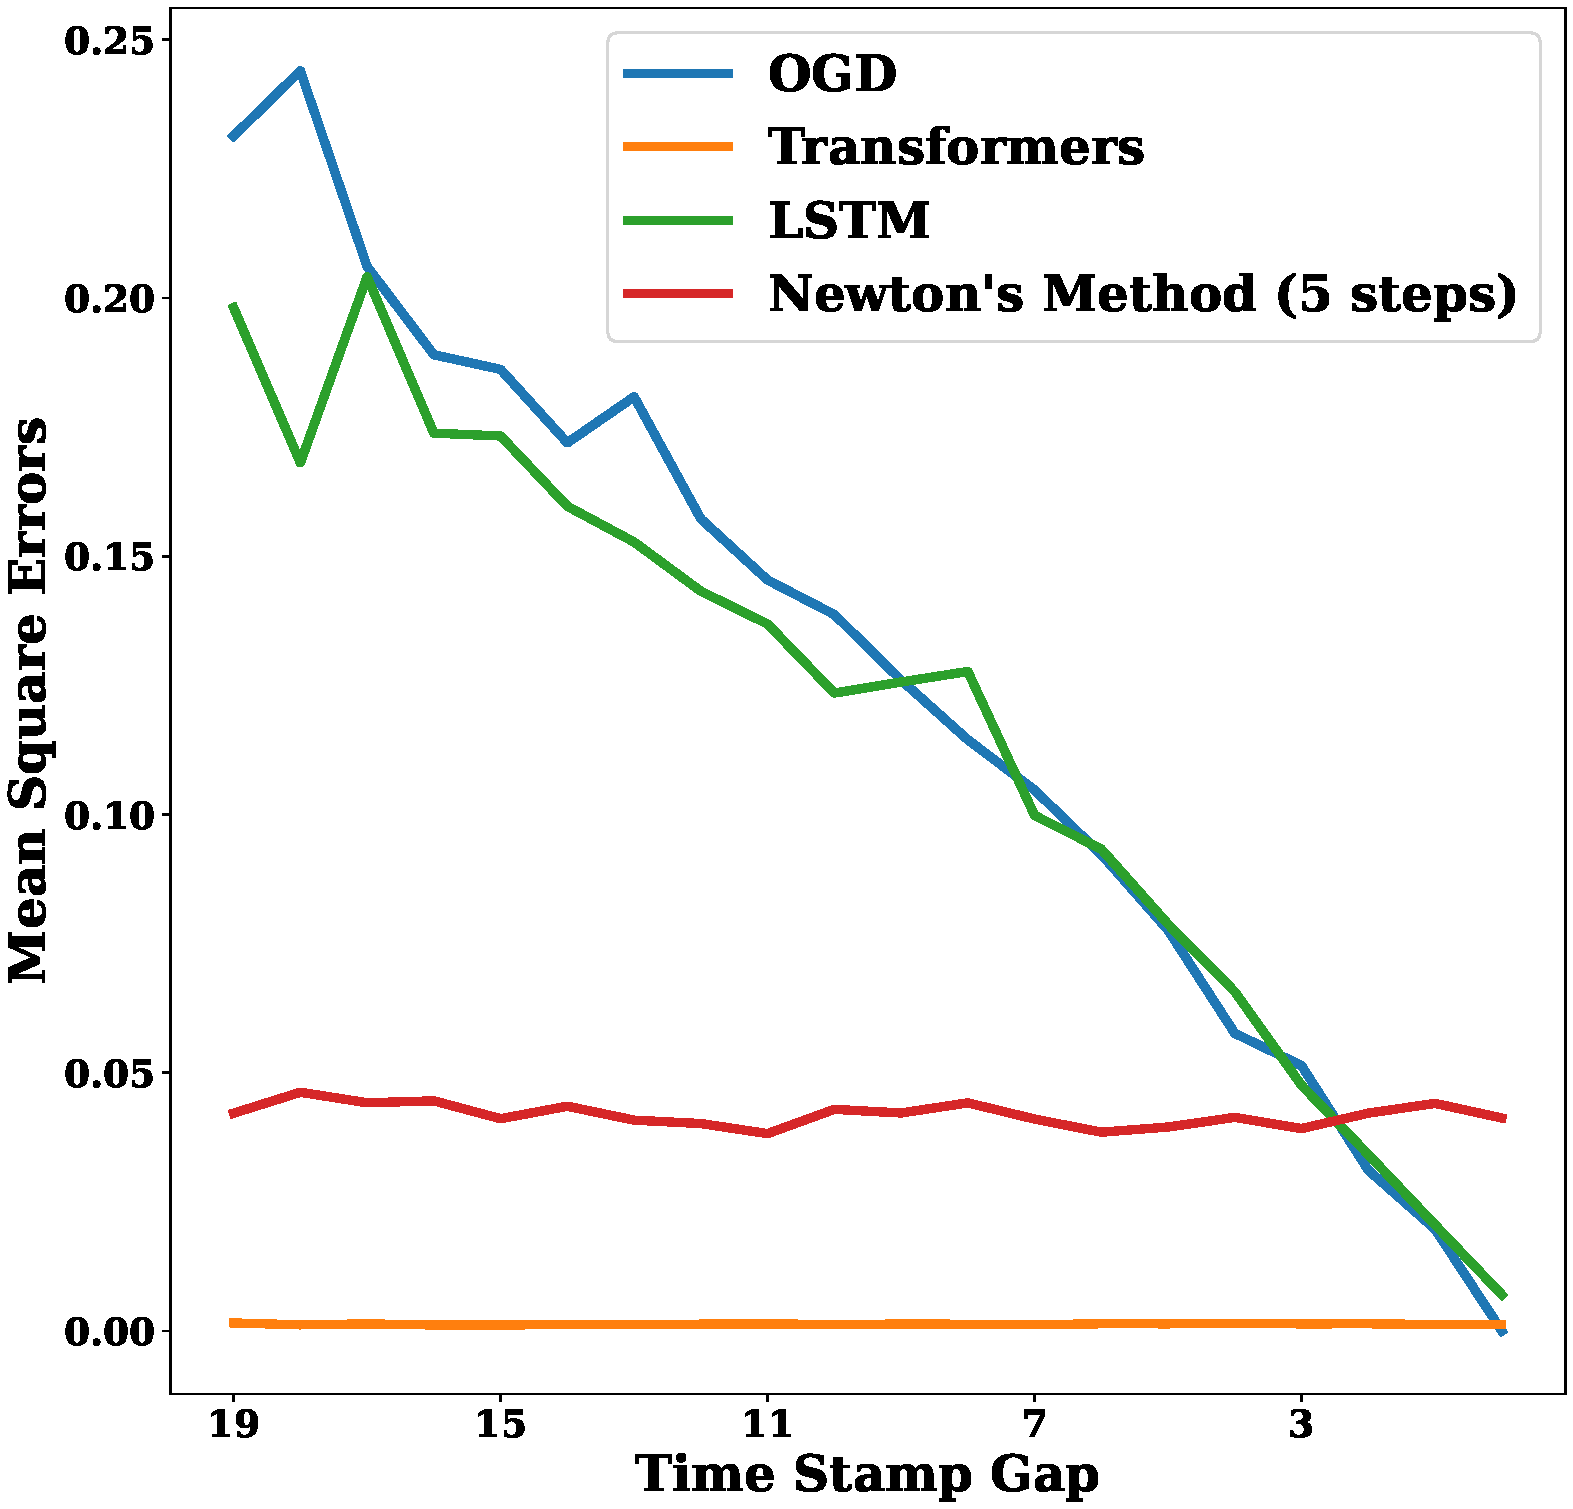
\includegraphics[width=0.43\linewidth]{Figures/forgetting.pdf}
    \caption{In the left figure, we measure model predictions with normalized MSE. Though LSTM is seemingly most similar to Newton's Method with only 5 steps, neither algorithm converges yet. OGD also has a similar trend as LSTM. In the right figure, we measure the model's error rate on example $\bx_{n-g}$ after seeing $n$ examples, for different values of the time stamp gap $g$ (see \cref{ssec:forgetting})}, and find both Transformers and not-converged Newton have better memorization than LSTM and OGD.
    \label{fig:lstm-experiment}
    \end{minipage}
\end{figure*}


% \begin{wrapfigure}[]{R}{0.3\textwidth}
% \vspace{-5mm}
%     \centering
%     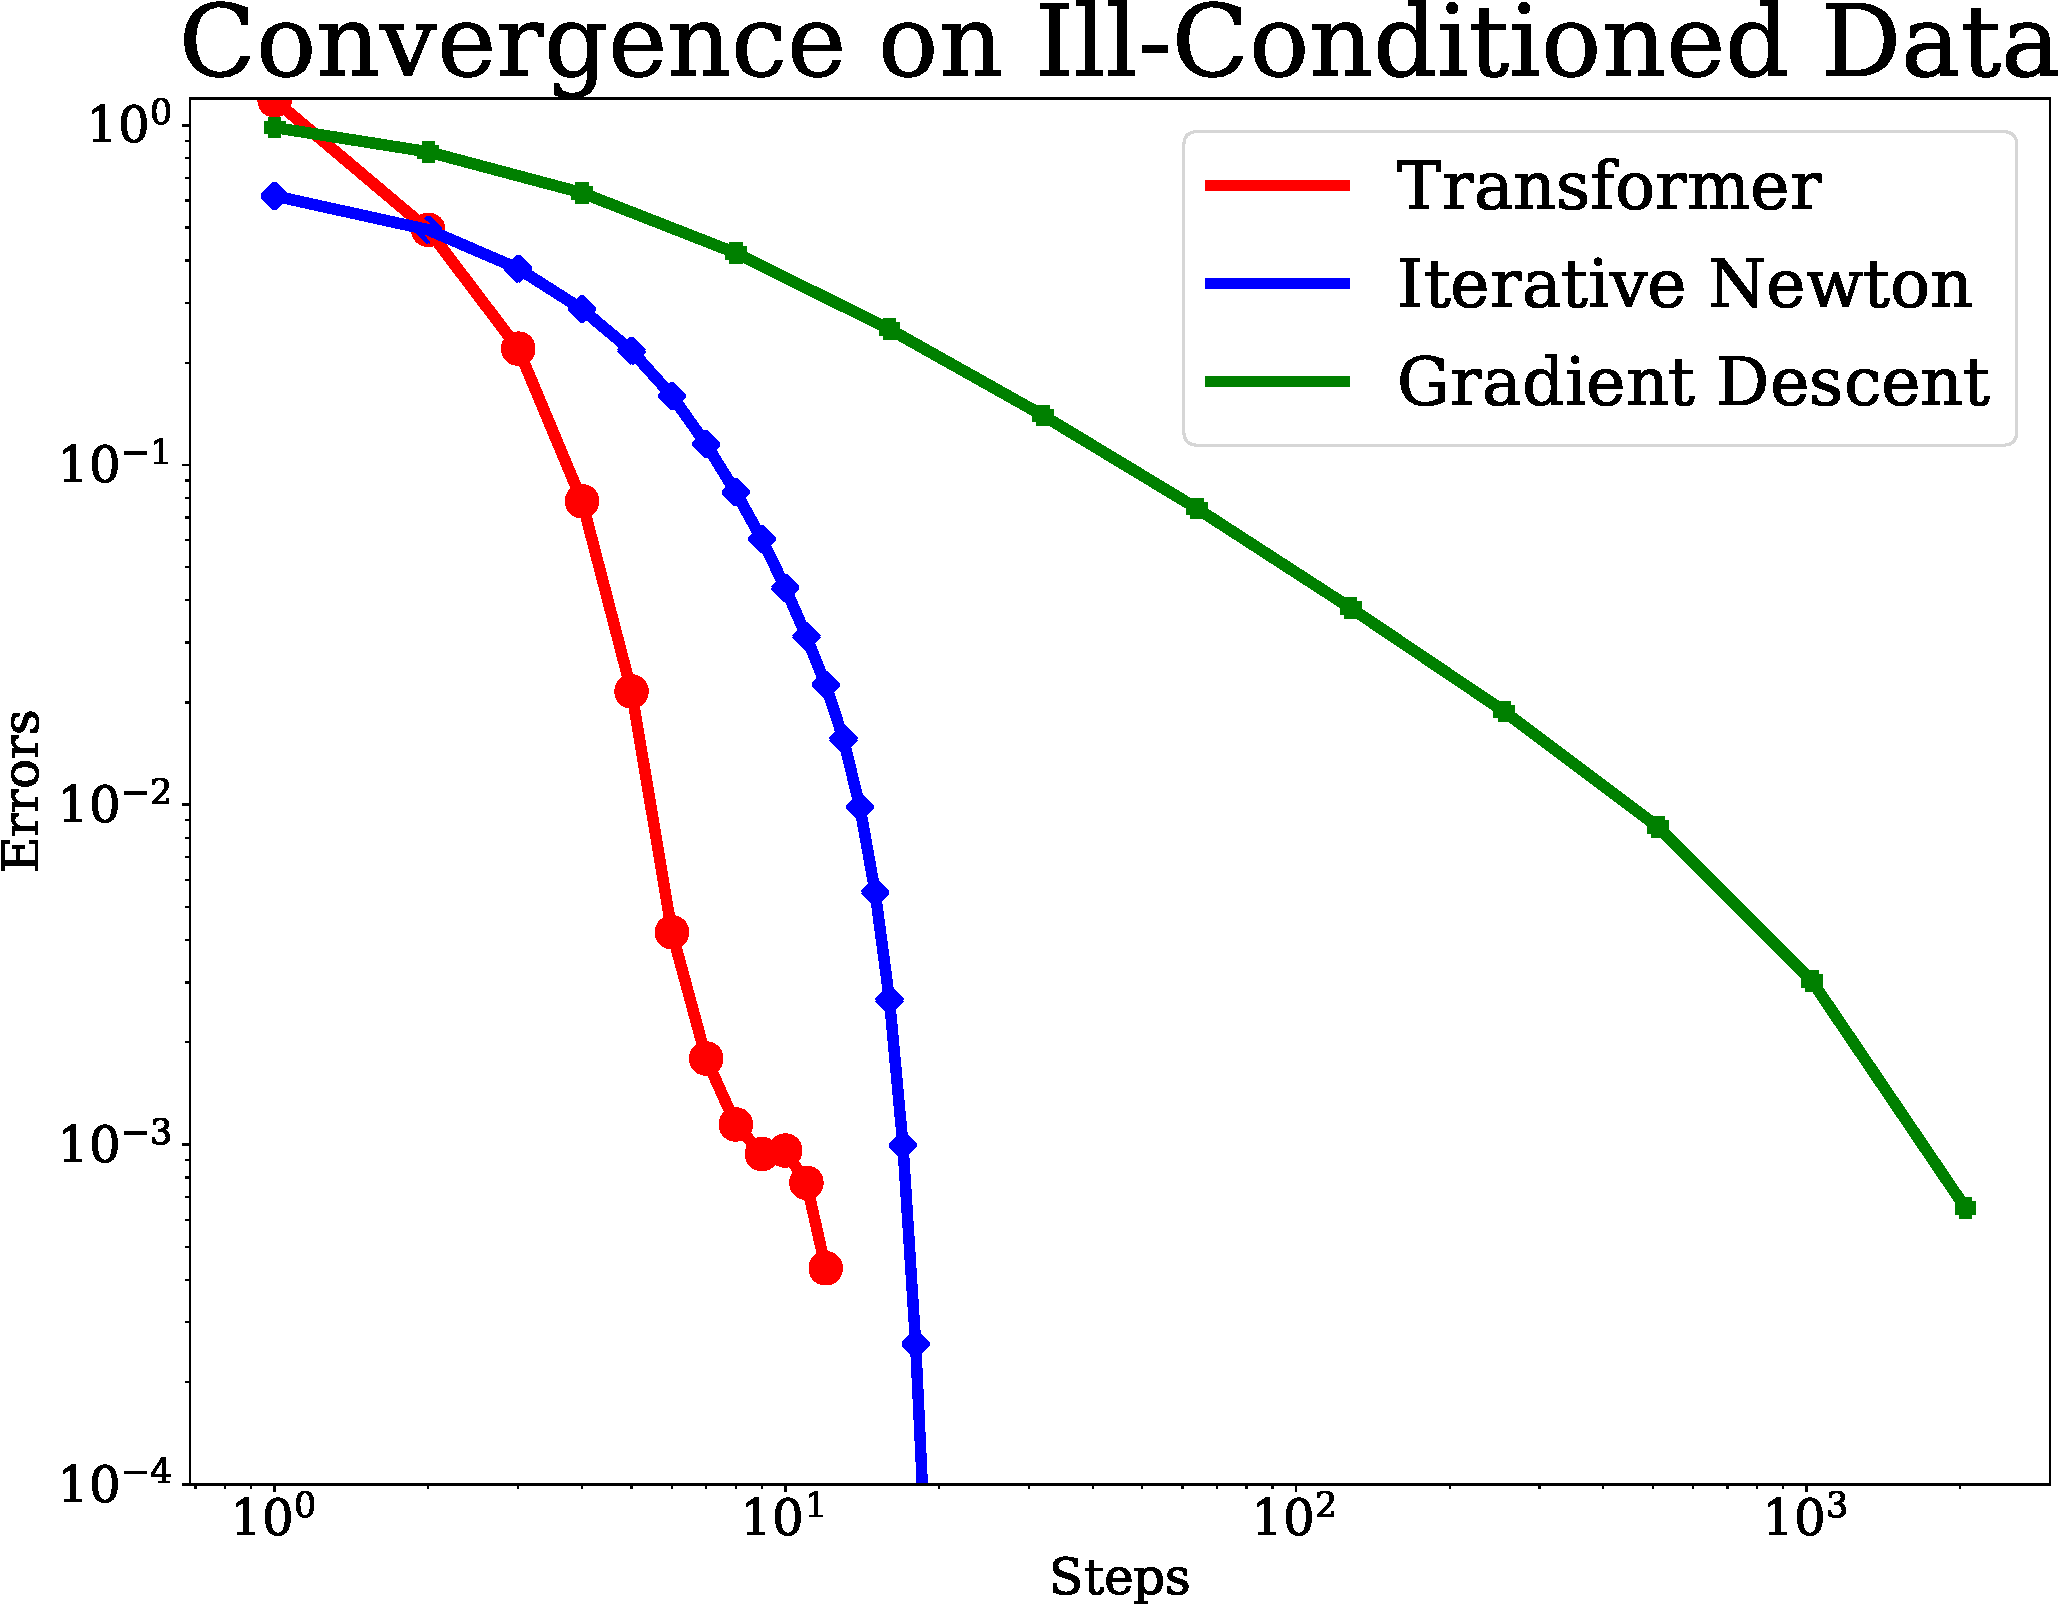
\includegraphics[width=\linewidth]{Figures/convergence/convergence_ill.pdf}
%     \caption{Transformers performance on ill-conditioned data. Both Transformers and \newton\ are able to converge to the OLS solution quickly whereas GD\ suffers.}
%     \label{fig:ill}
% \vspace{-5mm}
% \end{wrapfigure}

\vspace{-1mm}
\subsection{Transformers perform well on ill-conditioned data}  \label{ssec:ill}
\vspace{-1mm}
% \begin{figure}[t]
%     \centering
%     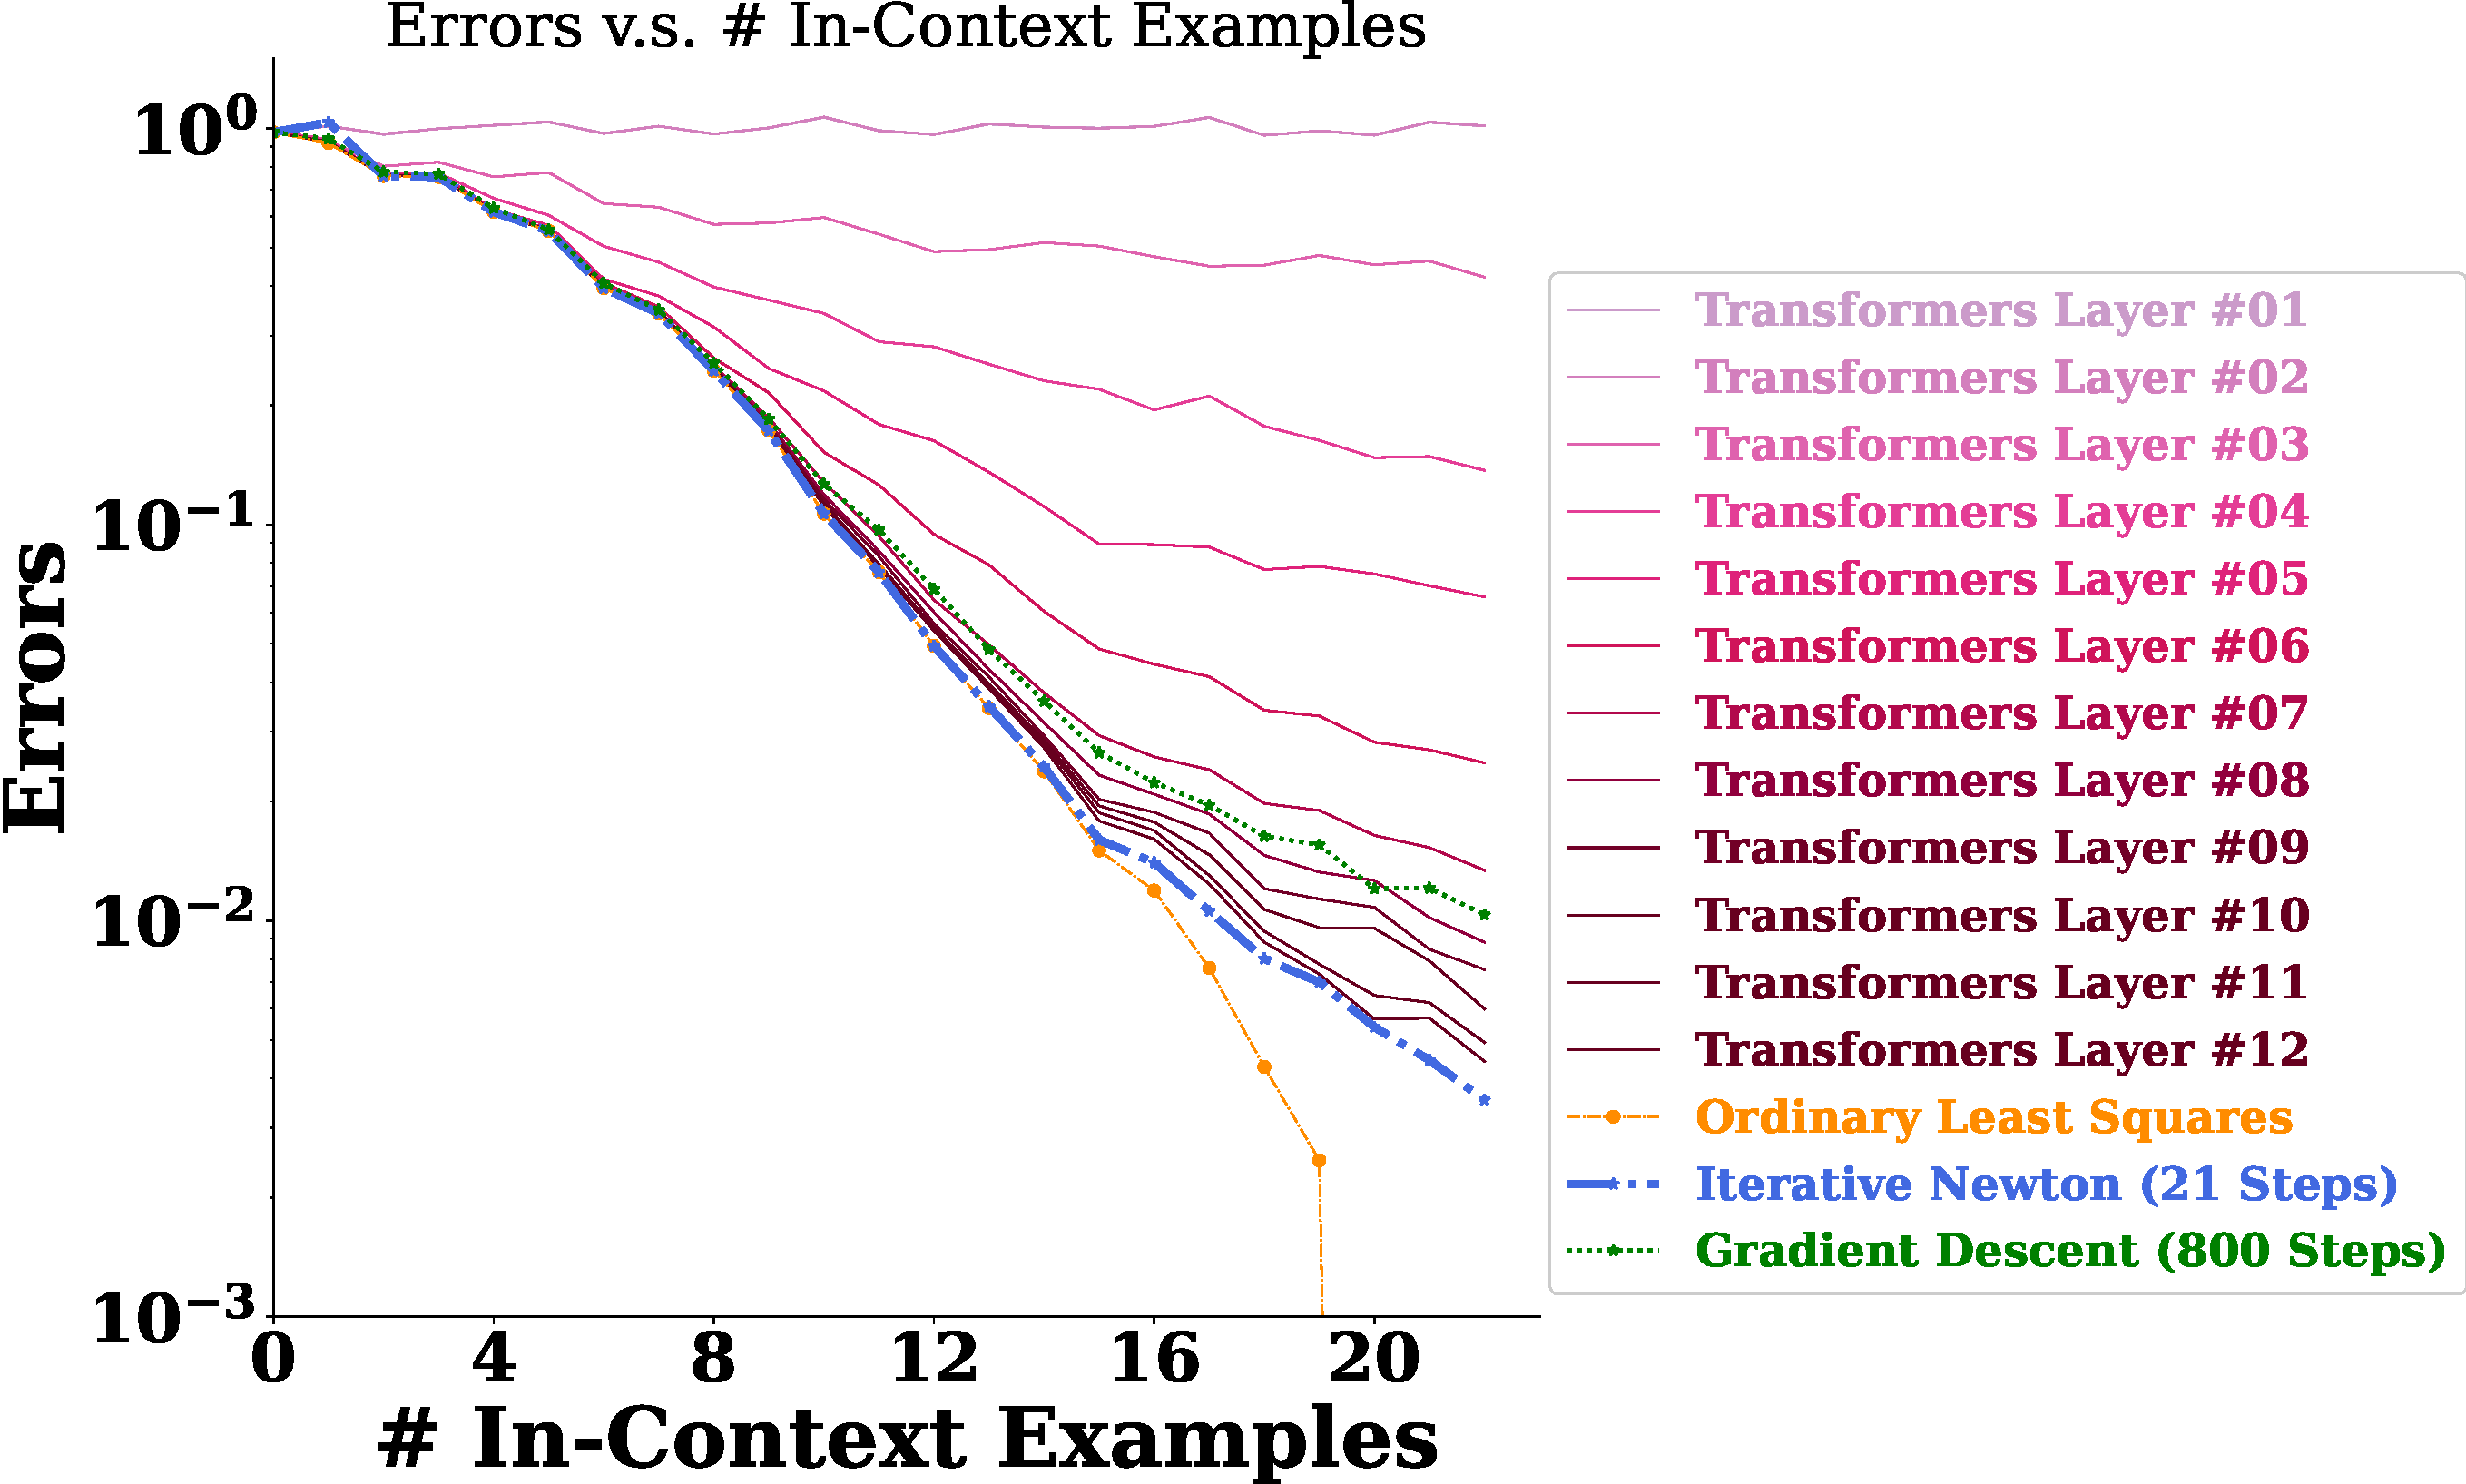
\includegraphics[width=0.8\linewidth]{Figures/progression/transformers_skew.pdf}
%     \caption{Transformers performance on ill-conditioned data. Both Transformers and \newton\ are able to converge to the OLS solution quickly whereas GD\ suffers.}
%     \label{fig:ill}
%     \vspace{-2ex}
% \end{figure}

\vspace{-1mm}


We repeat the same experiments with data $\bx_i \iid \mathcal N(\zero, \bSigma)$ sampled from an ill-condition covariance matrix $\bSigma$ with condition number $\kappa(\bSigma) = 100$, and eigenbasis chosen uniformly at random.  The first $d/2$ eigenvalues of $\bSigma$  are 100, and the last $d/2$ are 1. Note that choosing the eigenbasis uniformly at random for \emph{each} sequence ensures that there is a different covariance matrix $\bSigma$ for {each} sequence of datapoints.

As shown in \Cref{fig:ill}, the Transformer model's performance still closely matches \newton's Method with 21 iterations, same as when $\bSigma = \bI$ (see layer 10-12 in \Cref{fig:heatmap}). The convergence of second-order methods has a mild logarithmic dependence on the condition number since they correct for the curvature. On the other hand, GD's convergence is affected polynomially by conditioning.  %It's not hindered by the data distribution. 
As $\kappa(\bSigma)$ increase from 1 to 100, the number steps required for GD's convergence increases significantly (see Fig.~\ref{fig:ill} where GD requires 2,000 steps to converge), making it impossible for a 12-layer Transformers to implement these many gradient updates.  We also note that preconditioning the data by $(\bX^\top \bX)^\dagger$ can make the data well-conditioned, but since the eigenbasis is chosen uniformly at random, with high probability there is no sparse pre-conditioner or any fixed pre-conditioner which works across the data distribution. Computing $(\bX^\top \bX)^\dagger$ appears to be as hard as computing the OLS solution (Eq. \ref{eqn:obj})---in fact \citet{sharan2019memory} conjecture that first-order methods such as gradient descent and its variants cannot avoid polynomial dependencies in condition number in the ill-conditioned case.\footnote{Regarding preconditioning, we also note that---even for well-conditioned instances---preconditioned GD still gets a linear rate of convergence, whereas Transformers and \newton\ get superlinear rates.} 
See \Cref{app:ill} for detailed experiments on ill-conditioned problems. These experiments further strengthen our thesis that Transformers learn to perform second-order optimization methods in-context, not first-order methods such as GD. 

\subsection{Transformers Require $\mathcal O(d)$ Hidden Dimension}

We ablate 12-layer 1-head Transformers with various hidden sizes on $d=20$ problems. As shown in Figure \ref{fig:hiddien-dimension}, we observe that Transformers can mimic OLS solution when the hidden size is 32 or 64, but fail with smaller sizes. This resonates with our theoretical results on $\mathcal O(d)$ hidden dimension in Theorem \ref{thm:transformers_newton}, and in this case, the theorem ensures a construction of transformers to implement Iterative Newton's method. 
\begin{figure}[t]
    \centering
    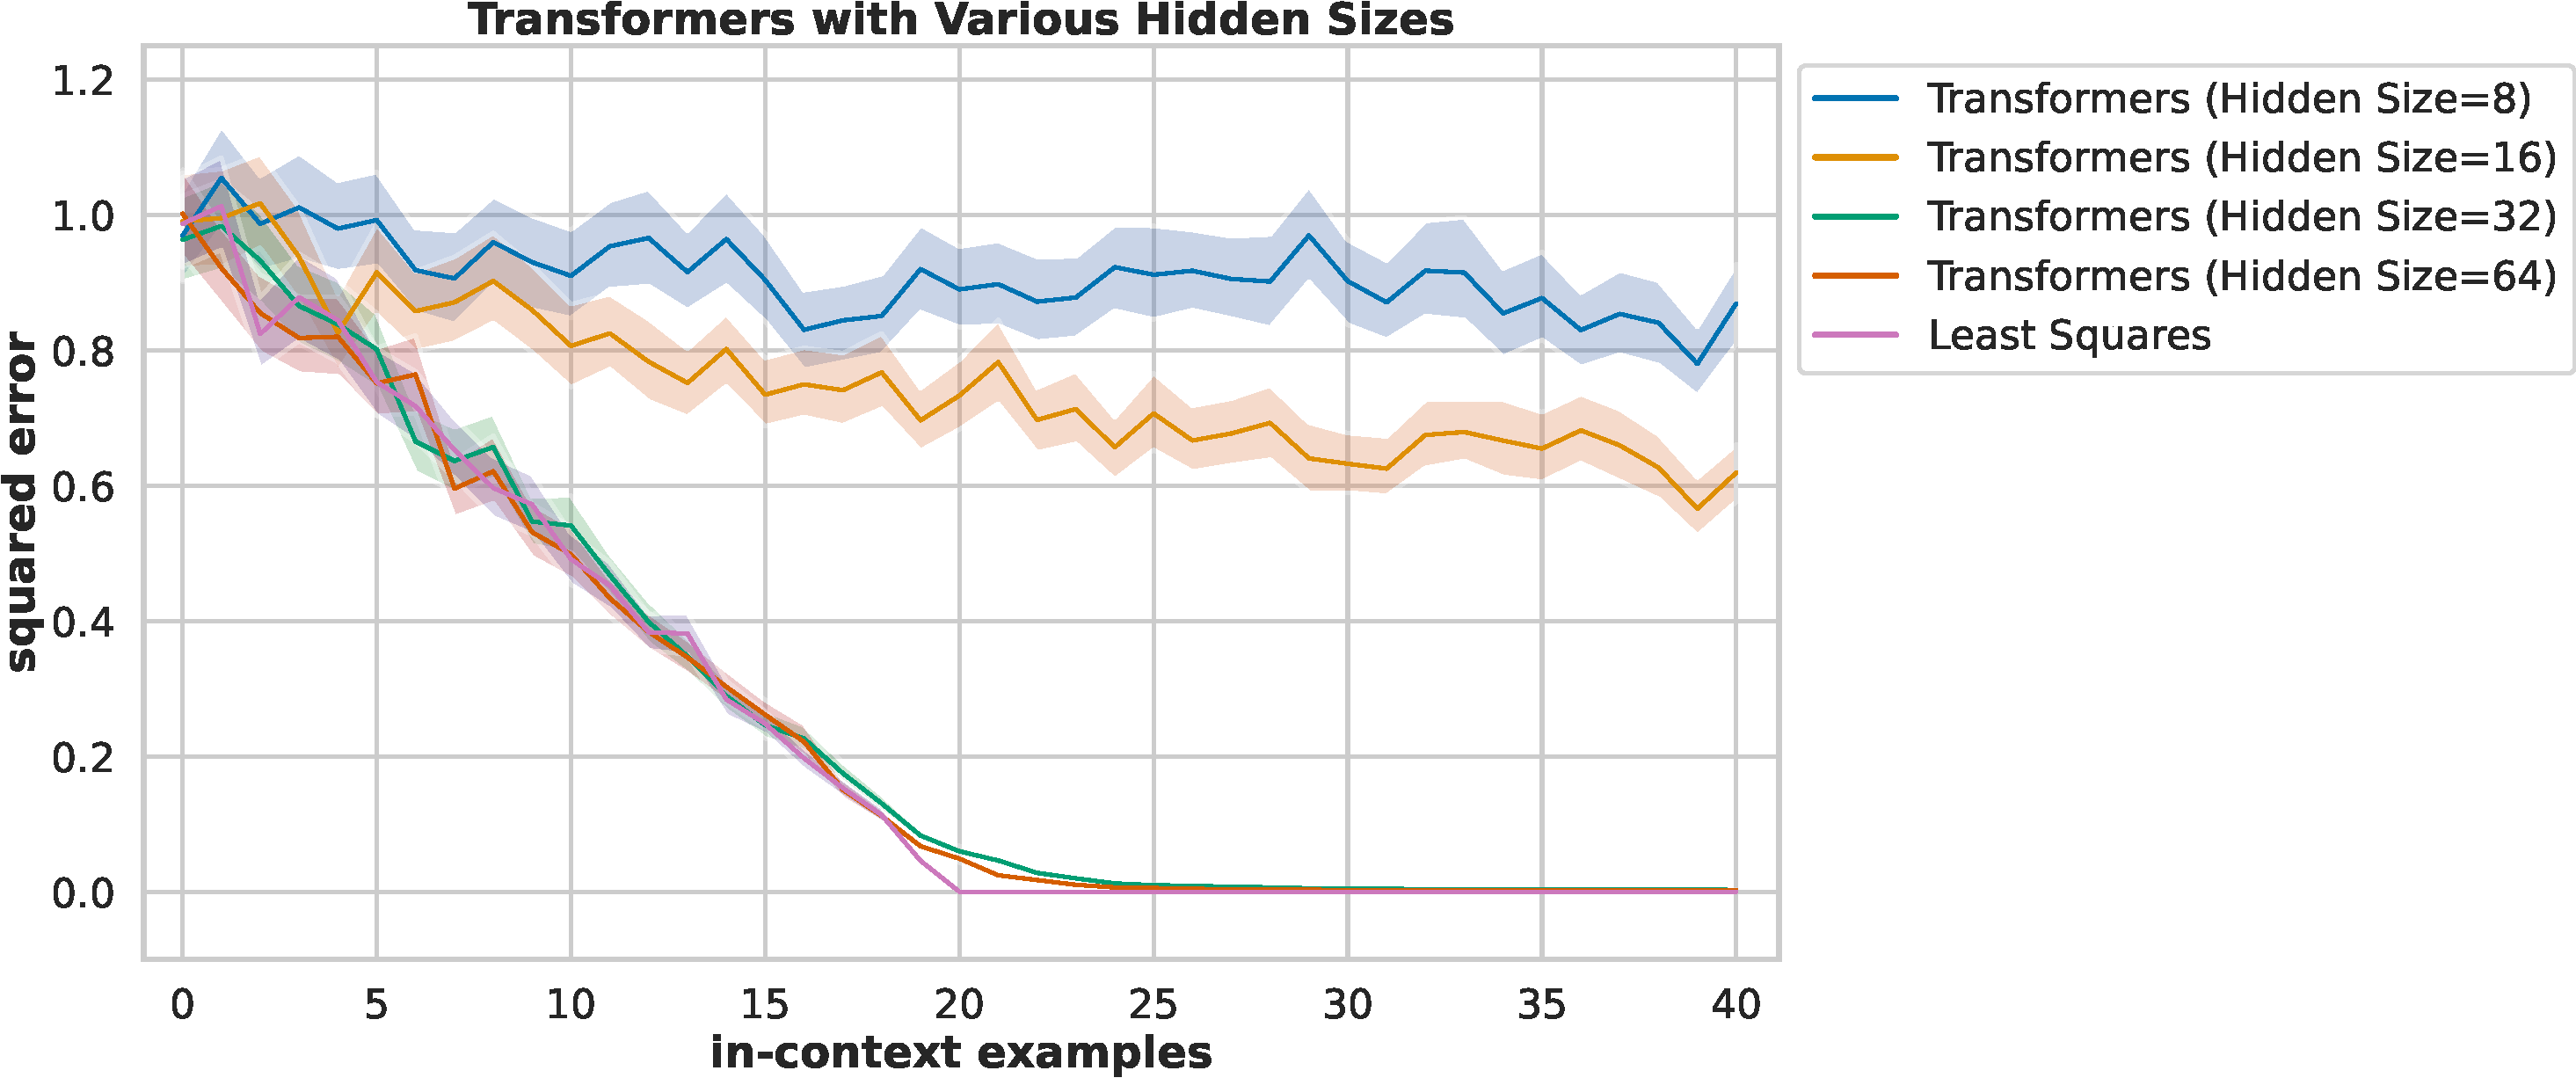
\includegraphics[width=0.75\linewidth]{Figures/linear_regression_hidden_size.pdf}
    \caption{Ablation on Transformer's Hidden Size. For linear regression problems with $d=20$, Transformers need $\mathcal O(d)$ hidden dimension to mimic OLS solutions.}
    \label{fig:hiddien-dimension}
\end{figure}


\vspace{-1mm}
\subsection{LSTM is more similar to OGD than Transformers} \label{ssec:lstm}
\vspace{-1mm}

As discussed in \S\ref{app:lstm}, LSTM is an alternative auto-regressive model widely used before the introduction of Transformers. 
Thus, a natural research question is: \textit{If Transformers can learn in-context, can LSTMs do so as well? If so, do they learn the same algorithms?} To answer this question, we train a LSTM model in an identical manner to the Transformers studied in the previous sections.

\Cref{fig:lstm-experiment} plots the error of Transformers, LSTMs, and other standard methods as a function of the number of in-context (i.e., training) examples provided.
While LSTMs can also learn linear regression in-context, they have much higher mean-squared error than Transformers.
Their error rate is similar to Iterative Newton's Method after only 5 iterations, a point where it is far from converging to the OLS solution.

Finally, we show that LSTMs behave more like an online learning algorithm than Transformers.
In particular, its predictions are biased towards getting more recent training examples correct, as opposed to earlier examples, as shown in \Cref{fig:lstm-experiment}.
This property makes LSTMs similar to online GD.
In contrast, five steps of Newton's method has the same error on average for recent and early examples, showing that the LSTM implements a very different algorithm from a few iterations of Newton.

We hypothesize that since LSTMs have limited memory, they must learn in a roughly online fashion;
in contrast, Transformer's attention heads can access the entire sequence of past examples, enabling it to learn more complex algorithms. See \S \ref{app:lstm} for more discussions.


